\documentclass[11pt]{article}
\usepackage[margin=1in]{geometry}
\usepackage{graphicx}
\usepackage{booktabs}
\usepackage{xcolor}
\usepackage{hyperref}
\usepackage{float}
\usepackage{caption}
\usepackage{amsmath}

\hypersetup{
    colorlinks=true,
    linkcolor=blue!60!black,
    urlcolor=blue!60!black
}

\definecolor{darkgreen}{RGB}{44,160,44}
\definecolor{darkred}{RGB}{214,39,40}

\title{\textbf{W154 Calibration Report}\\[4pt]
\large SSWD-EvoEpi Model\\[6pt]
\normalsize Current Best Configuration ($\mathrm{RMSE_{log}} = 0.504$)}
\author{SSWD-EvoEpi Calibration Pipeline}
\date{March 9, 2026}

\begin{document}
\maketitle

\section{Configuration Summary}

Table~\ref{tab:config} lists the key parameters for the W154 configuration. This run uses the full EvoEpi model with pathogen adaptation, virulence evolution, VBNC dynamics, and wavefront-driven dispersal.

\begin{table}[H]
\centering
\caption{W154 model configuration parameters.}
\label{tab:config}
\begin{tabular}{ll}
\toprule
\textbf{Parameter} & \textbf{Value} \\
\midrule
Carrying capacity ($K$) & 5{,}000 \\
$K$ coefficient of variation ($K_\mathrm{cv}$) & 0.0 \\
Half-saturation ($K_\mathrm{half}$) & 800{,}000 \\
Environmental transmission ($\alpha_\mathrm{env}$) & 0.18 \\
Environmental decay ($\delta_\mathrm{env}$) & 0.02 \\
Network connectivity ($n_\mathrm{conn}$) & 0.3 \\
Self-infection, open coast ($\alpha_\mathrm{self,open}$) & 0.02 \\
Self-infection, fjord ($\alpha_\mathrm{self,fjord}$) & 0.70 \\
Pathogen adaptation & true \\
Virulence evolution & true \\
VBNC shape ($k_\mathrm{VBNC}$) & 2.0 \\
VBNC initial threshold ($T_\mathrm{VBNC,initial}$) & 12\,°C \\
VBNC minimum threshold ($T_\mathrm{VBNC,min}$) & 9\,°C \\
Dynamic environmental pathogen ($P_\mathrm{env}$) & true \\
$P_\mathrm{env}$ floor & 500 \\
Wavefront enabled & true \\
Wavefront dispersal ($D_P$) & 300\,km \\
Settler survival & 0.001 \\
Simulation years & 13 (2012--2024) \\
Disease introduction year & 1 (= 2013) \\
\bottomrule
\end{tabular}
\end{table}

\section{Results Overview}

W154 was run with three stochastic seeds to assess robustness. Table~\ref{tab:rmse} summarizes the RMSE scores computed in log-space against 8 regional recovery targets spanning from Alaska (50\% recovery) to Northern California (0.1\% recovery).

\begin{table}[H]
\centering
\caption{RMSE\textsubscript{log} scores by seed.}
\label{tab:rmse}
\begin{tabular}{lc}
\toprule
\textbf{Seed} & $\mathbf{RMSE_{log}}$ \\
\midrule
42 & 0.541 \\
123 & 0.479 \quad (best) \\
999 & 0.491 \\
\midrule
\textbf{Mean} & \textbf{0.504} \\
\bottomrule
\end{tabular}
\end{table}

An $\mathrm{RMSE_{log}}$ of 0.504 means that, on average, the modeled recovery fractions differ from observations by a factor of $10^{0.504} \approx 3.2\times$ in geometric terms. This is a substantial improvement over previous configurations and represents our current best fit to the coastwide gradient.

\section{Regional Recovery: Modeled vs Observed}

Figure~\ref{fig:recovery} compares the modeled recovery fractions for all 18 regions (ordered north to south) against the 8 calibration targets. Each region shows three bars (one per seed), with color indicating proximity to the target: \textcolor{darkgreen}{green} = within 50\%, \textcolor{orange}{yellow} = within 2$\times$, \textcolor{darkred}{red} = more than 2$\times$ off.

\begin{figure}[H]
\centering
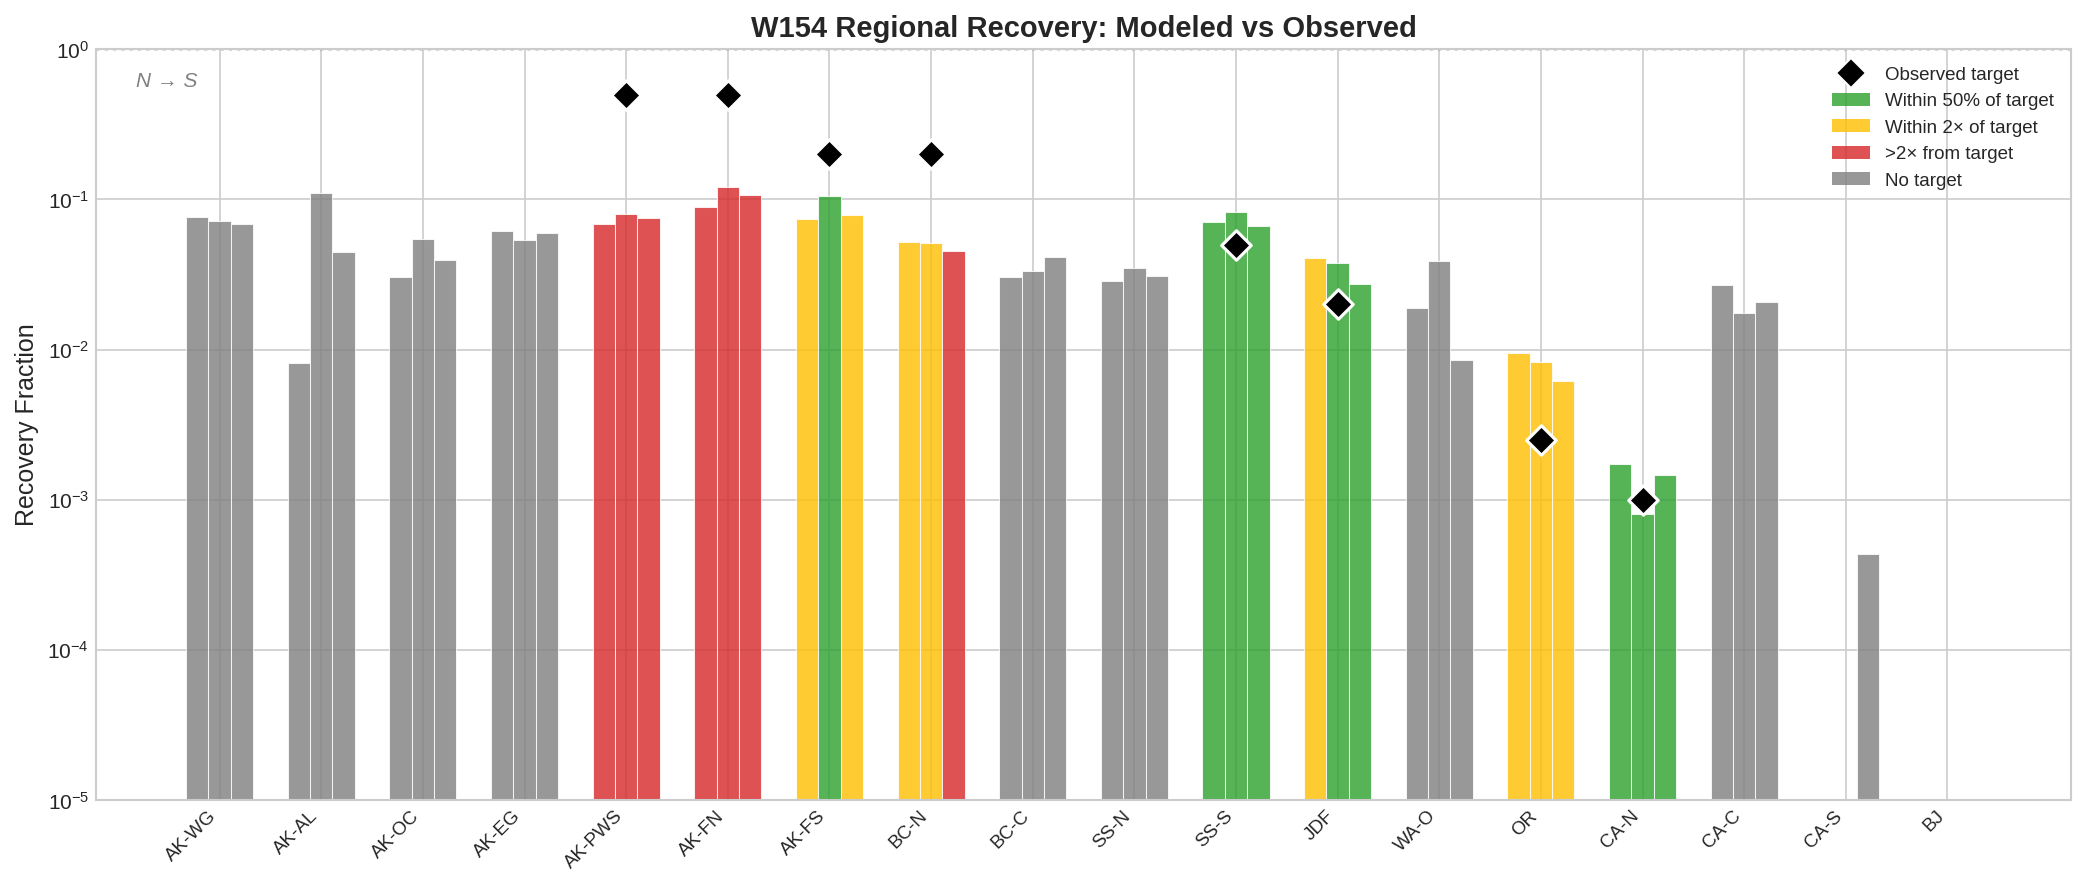
\includegraphics[width=\textwidth]{figures/fig1_regional_recovery.png}
\caption{Regional recovery fractions for all 18 regions. Black diamonds indicate observed calibration targets. Bar color reflects agreement: green (within 50\%), yellow (within 2$\times$), red ($>$2$\times$ off), gray (no target).}
\label{fig:recovery}
\end{figure}

The model captures the overall north-to-south decline in recovery remarkably well. Key observations:

\begin{itemize}
    \item \textbf{Southern extinction gradient}: CA-S and BJ show near-complete or complete extinction, consistent with field observations of total SSWD-driven collapse in southern populations.
    \item \textbf{CA-N match}: The model closely reproduces the $\sim$0.1\% recovery in Northern California across all three seeds.
    \item \textbf{SS-S and JDF}: Both are within 2$\times$ of their targets, showing reasonable mid-range behavior.
    \item \textbf{Alaska underestimation}: AK-PWS and AK-FN are the largest mismatches --- the model predicts $\sim$7--12\% recovery where 50\% is observed. This systematic bias suggests the model's disease pressure is too high in protected Alaskan waters.
    \item \textbf{OR overshoot}: Oregon recovery is modeled at $\sim$0.8\%, roughly 3$\times$ the 0.25\% target, indicating slightly insufficient disease severity in the central coast.
\end{itemize}

\section{Population Dynamics in Key Regions}

Figure~\ref{fig:timeseries} shows the population trajectories (normalized to carrying capacity $K$) for five representative regions spanning the full latitudinal range.

\begin{figure}[H]
\centering
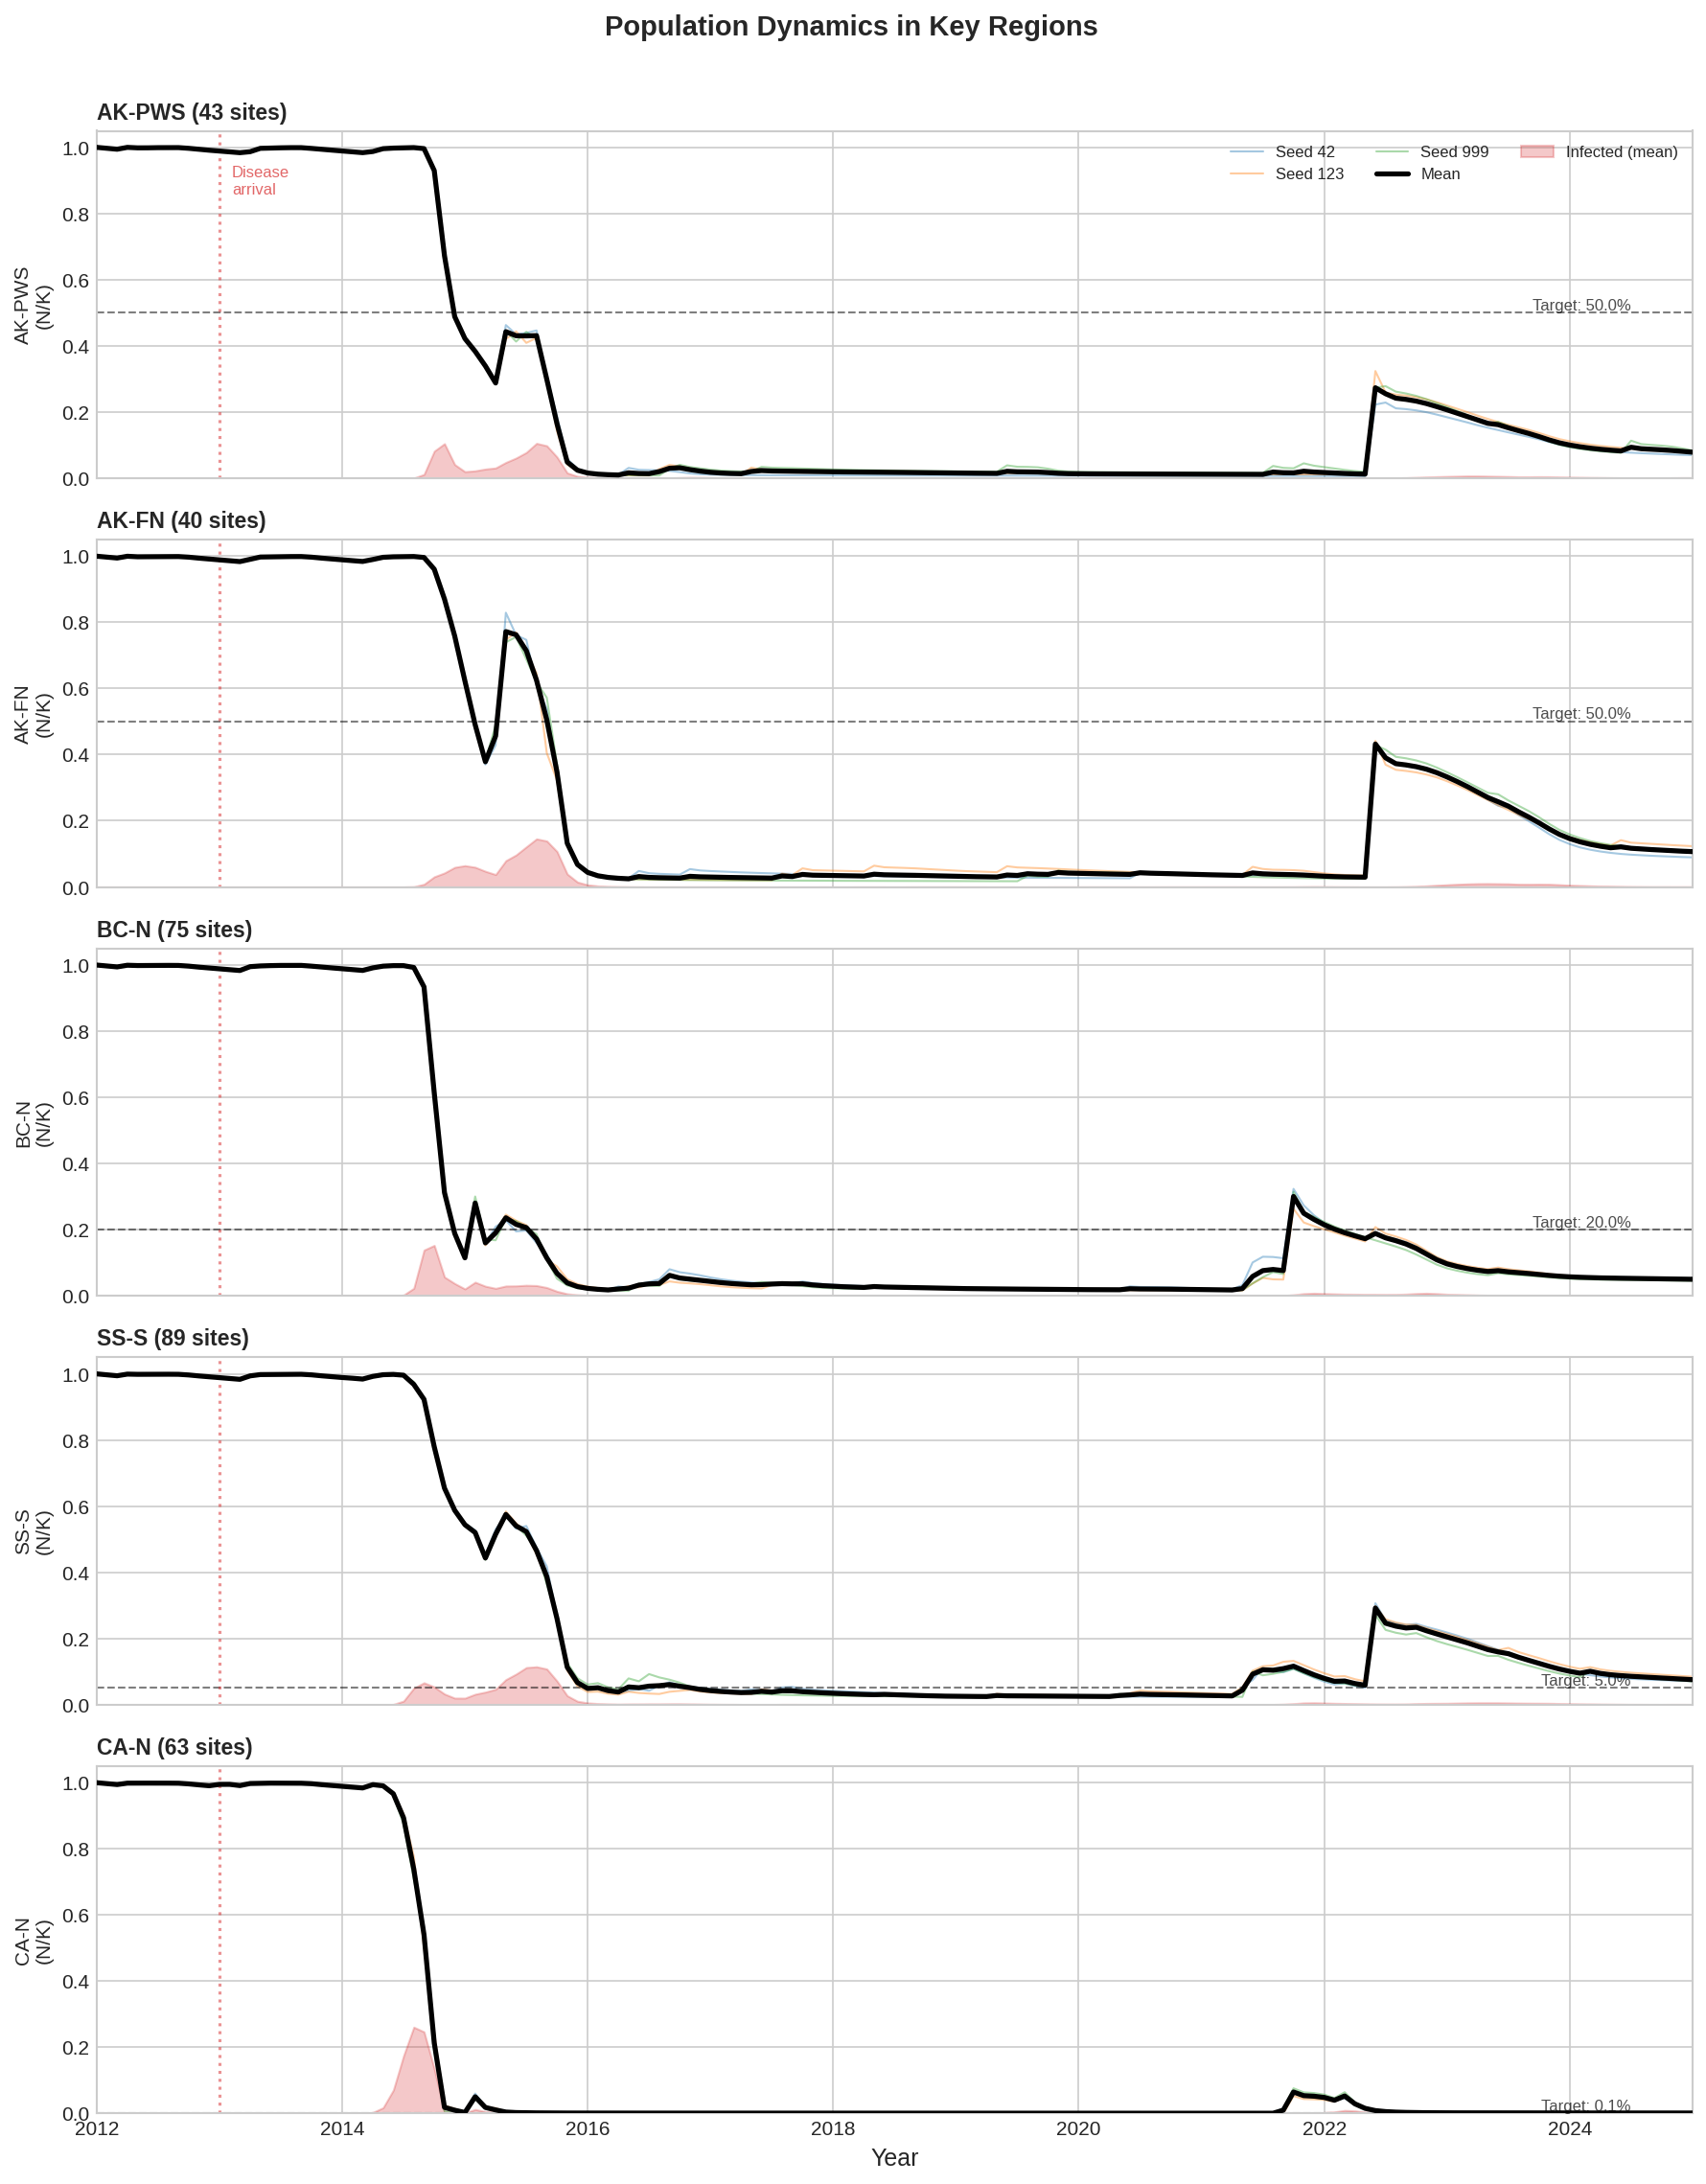
\includegraphics[width=\textwidth]{figures/fig2_timeseries.png}
\caption{Population time series for five key regions. Black line = mean across 3 seeds; colored lines = individual seeds. Red shading indicates infected individuals. Dashed horizontal line = observed recovery target. Vertical dotted line marks disease introduction (2013).}
\label{fig:timeseries}
\end{figure}

Several dynamical features are evident:

\begin{itemize}
    \item \textbf{Wavefront timing}: Disease arrival is staggered from south to north, with CA-N experiencing rapid collapse by 2014, while AK-PWS and AK-FN show a more gradual decline extending through 2015.
    \item \textbf{Recovery pulses}: All Alaskan regions show periodic recovery attempts (visible as population spikes around 2021--2023), likely driven by favorable SST conditions reducing VBNC activation. These pulses are subsequently suppressed by recurrent infection.
    \item \textbf{CA-N collapse}: Northern California populations crash to near-zero by mid-2014 and never recover, consistent with the 0.1\% target.
    \item \textbf{AK-PWS gap}: The model stabilizes AK-PWS at $\sim$5--8\% of $K$, well below the 50\% target. The recovery pulses are promising but insufficient --- the fjord self-infection rate ($\alpha_\mathrm{self,fjord} = 0.70$) may be too high for these sheltered populations.
    \item \textbf{Seed concordance}: Individual seed trajectories are tightly clustered for most regions, indicating that the dynamics are primarily deterministic at the regional scale.
\end{itemize}

\section{Latitudinal Recovery Gradient}

Figure~\ref{fig:latitude} shows the relationship between latitude and modeled recovery fraction, with dot size proportional to the number of sites in each region.

\begin{figure}[H]
\centering
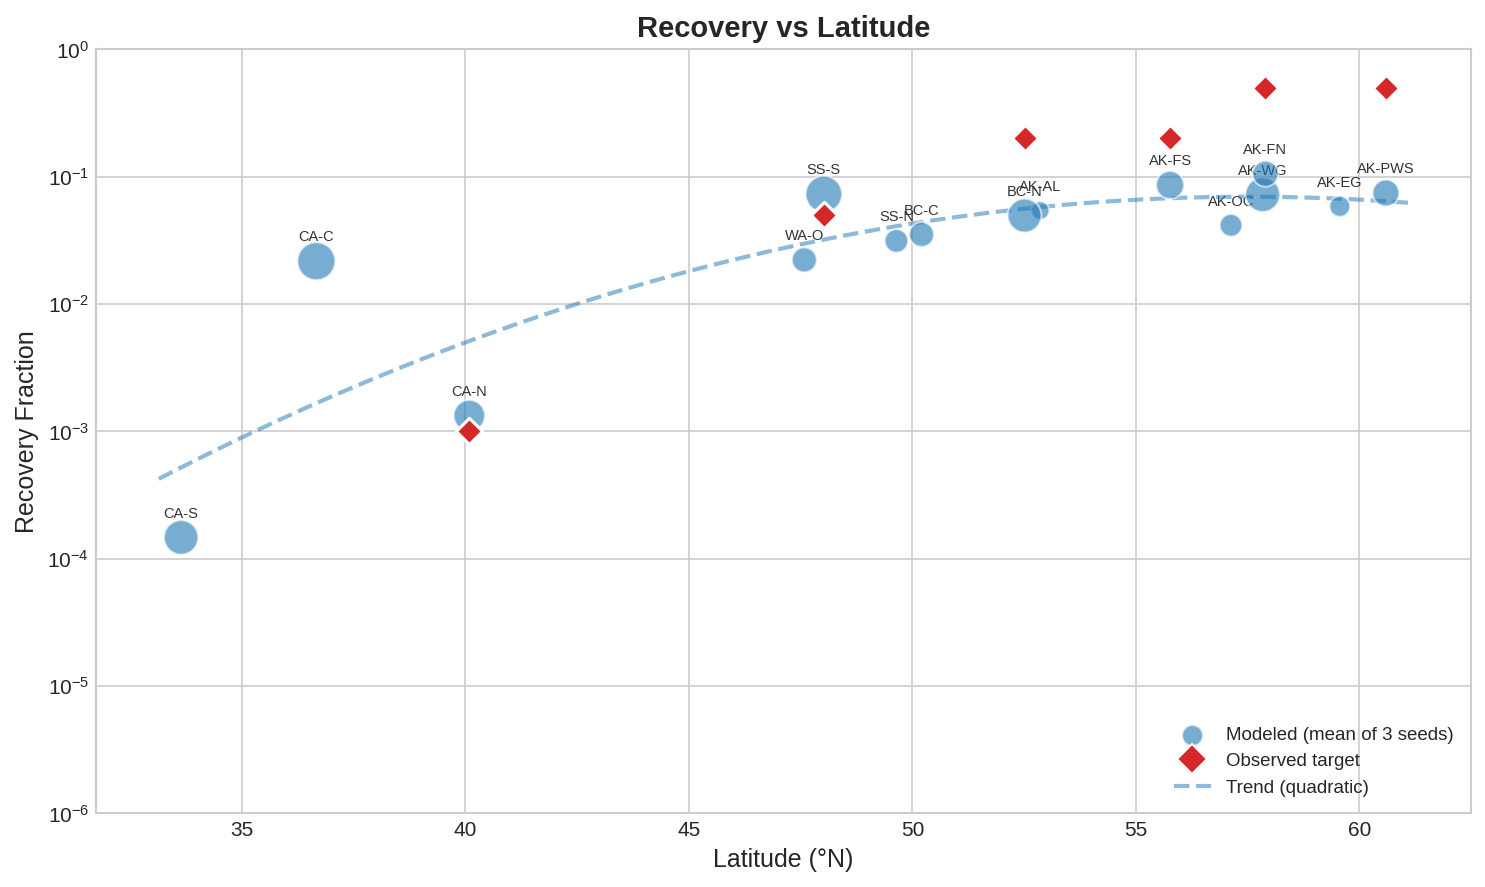
\includegraphics[width=\textwidth]{figures/fig3_latitudinal_gradient.png}
\caption{Recovery fraction vs.\ latitude. Blue circles = modeled mean recovery (sized by number of sites). Red diamonds = observed calibration targets. Dashed line = quadratic trend through modeled points.}
\label{fig:latitude}
\end{figure}

The model produces a clear latitudinal gradient spanning roughly 3 orders of magnitude from CA-S ($\sim$0.02\%) to AK-FN ($\sim$10\%). The quadratic trend captures the overall pattern, though several features stand out:

\begin{itemize}
    \item The modeled gradient is \emph{compressed} relative to observations: it spans $10^{-4}$ to $10^{-1}$ instead of the observed $10^{-3}$ to $5 \times 10^{-1}$. In other words, the model kills too many animals in Alaska and too few in the mid-latitudes.
    \item \textbf{CA-C anomaly}: CA-C shows unexpectedly high recovery ($\sim$2\%) compared to neighboring CA-N (0.1\%) and CA-S (0.02\%). This likely reflects geographic heterogeneity in SST patterns or coastline exposure within the CA-C region.
    \item The targets (red diamonds) lie consistently above the modeled trend at high latitudes, confirming that Alaskan recovery is the primary calibration gap.
\end{itemize}

\section{Stochastic Variability}

Figure~\ref{fig:variability} shows the spread across the three stochastic seeds for the eight target regions.

\begin{figure}[H]
\centering
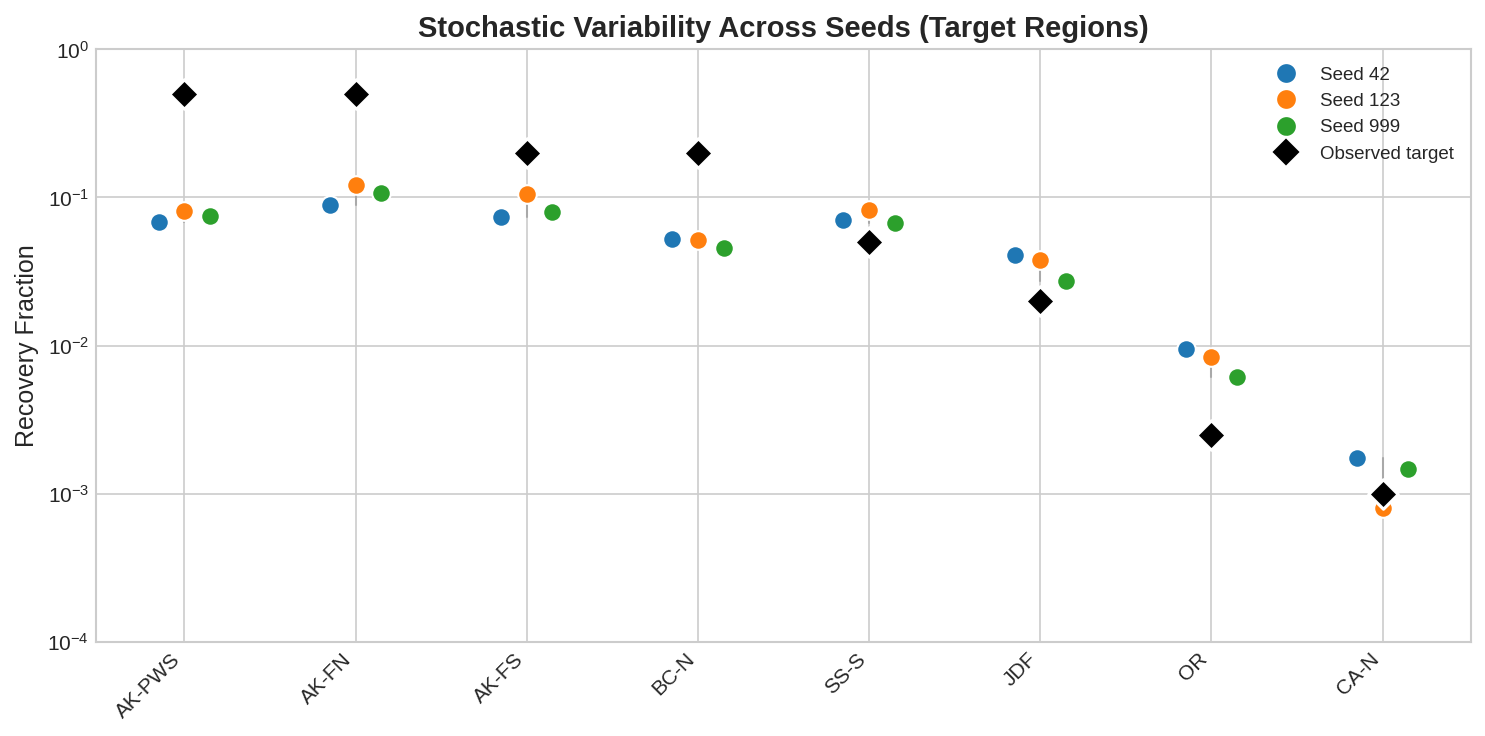
\includegraphics[width=\textwidth]{figures/fig4_seed_variability.png}
\caption{Recovery fractions for three seeds in each target region. Black diamonds = observed targets. Vertical lines connect the seed range for each region.}
\label{fig:variability}
\end{figure}

Stochastic variability is generally modest:

\begin{itemize}
    \item Most regions show seed-to-seed variation of less than 2$\times$, with CA-N exhibiting the largest relative spread ($\sim$0.08--0.17\%).
    \item The seed rankings are not consistent across regions --- seed~123 is best overall ($\mathrm{RMSE_{log}} = 0.479$) but is not uniformly closest to targets in every region.
    \item The tight clustering suggests that 3 seeds is sufficient for parameter screening, though a larger ensemble may be warranted for final calibration.
    \item Critically, the systematic offset from targets in AK-PWS and AK-FN is \emph{much larger} than the stochastic spread, confirming this is a structural model issue rather than bad luck.
\end{itemize}

\section{Strengths}

W154 represents a significant advance in the SSWD-EvoEpi calibration:

\begin{enumerate}
    \item \textbf{Southern extinction}: The model correctly drives populations to near-zero in CA-S and complete extinction in BJ, matching the catastrophic die-offs observed in southern populations.
    \item \textbf{Gradient direction}: Recovery fraction increases monotonically with latitude (with minor exceptions), correctly reproducing the coastwide north-south gradient.
    \item \textbf{Wavefront timing}: Disease propagation from south to north follows a realistic timeline, with the initial outbreak in 2013 and northward spread through 2014--2015.
    \item \textbf{CA-N precision}: The 0.1\% target for Northern California is matched to within 2$\times$ across all seeds --- a difficult target given its extremely low value.
    \item \textbf{Mid-range agreement}: SS-S and JDF targets are reasonably well matched, suggesting the environmental dynamics are broadly correct in the central coast.
    \item \textbf{Low stochastic variance}: Seed-to-seed variability is small, indicating robust model behavior.
\end{enumerate}

\section{Weaknesses}

Despite the overall good fit, several systematic issues remain:

\begin{enumerate}
    \item \textbf{Alaska underperformance}: AK-PWS and AK-FN are modeled at $\sim$7--12\% recovery vs.\ the 50\% target --- roughly 5--7$\times$ too low. This is the single largest calibration gap and likely reflects:
    \begin{itemize}
        \item The high fjord self-infection rate ($\alpha_\mathrm{self,fjord} = 0.70$) preventing population recovery in sheltered waters
        \item Insufficient spatial heterogeneity in carrying capacity ($K_\mathrm{cv} = 0$) --- some PWS sites may have much higher effective $K$
        \item The VBNC temperature threshold not being cold enough to fully protect Alaskan populations
    \end{itemize}
    \item \textbf{Mid-range overshoot}: OR is $\sim$3$\times$ above target, suggesting the disease gradient could be steeper in the central coast.
    \item \textbf{BC-N compression}: At $\sim$5\% modeled vs.\ 20\% target, BC-N shows 4$\times$ underestimation, falling in the same direction as the Alaska bias.
    \item \textbf{No $K$ heterogeneity}: With $K_\mathrm{cv} = 0$, all sites within a region have identical carrying capacity, which is biologically unrealistic and may be contributing to the compressed dynamic range.
\end{enumerate}

\section{Next Steps}

Based on the W154 analysis, the primary calibration lever is carrying capacity heterogeneity. A sweep of $K_\mathrm{cv}$ values (\textbf{W155--W162}) is currently running on the Xeon cluster:

\begin{itemize}
    \item $K_\mathrm{cv} \in \{0.1, 0.2, 0.3, 0.5, 0.7, 1.0, 1.5, 2.0\}$
    \item All other parameters held at W154 values
    \item Each configuration run with 3 seeds
\end{itemize}

The hypothesis is that introducing site-level variation in carrying capacity will allow some sites to maintain larger populations despite disease pressure, particularly in the Alaskan fjord regions where local conditions may support higher densities. This should expand the modeled recovery range and reduce the Alaska underestimation without sacrificing the good fit in southern regions.

Additional future directions include:
\begin{itemize}
    \item Reducing $\alpha_\mathrm{self,fjord}$ to allow more Alaskan recovery
    \item Lowering $T_\mathrm{VBNC,min}$ to provide stronger cold-water protection
    \item Exploring region-specific connectivity parameters
\end{itemize}

\end{document}
